\documentclass[a4paper,12pt]{article}
%For links
%\usepackage{url}
%For images
\usepackage{graphicx}
\begin{document}
\begin{enumerate}
    \item $$sin(2x)=0.875$$
    Med en miniräknare tar man $sin^{-1}$ på båda sidorna och räknar ut
    $$2x=sin^{-1}(0.875)\Rightarrow x=sin^{-1}(0.875)/2\approx 0.533$$

    Så för alla blir det ungefär $0.533+2\pi n, n\in \mathbf{Z}$. 
    Rent geometriskt kan det beskrivas nedan. 
    Det gör det även självklart
    att det andra svaret inom $0 \leq x \leq \pi$ är $\pi-x\approx=2,61$ som ligger till vänster om bilden.

    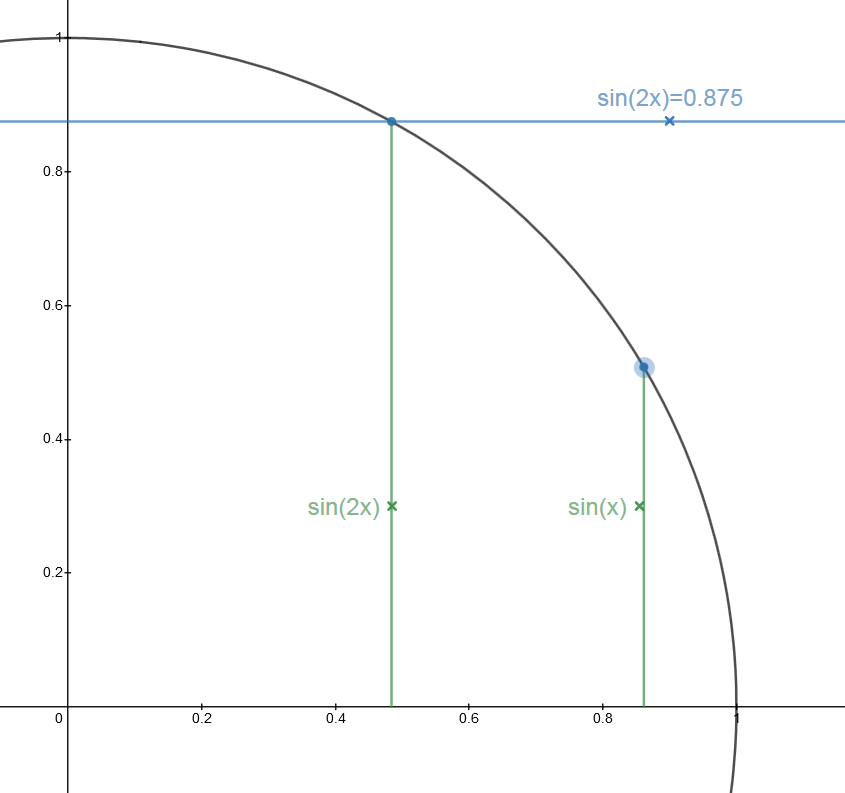
\includegraphics[scale=0.45]{Figur1.png}
    
    \item 
    \begin{enumerate}
        \item Med ren spekulation, 2.5 är mindre än pi men mer än pi/2, så det måste vara i andra kvadranten. 
        Vi vet att $\pi=180^\circ $. Vi kan nu ta fram det med
        hjälp av enhetsanalys. Om 180 är grader per radie, och pi är endast ett nummer, och v är en vinkel
        i grader, så kommer vi få $v\pi / 180$ som svar. Räknar man ut enheterna får man radien.
        
        \item Vi sätter in det som v i ekvationen och vi får $36\pi / 180 = 9 \pi/ 45$
    \end{enumerate}


    \begin{enumerate}
        \item 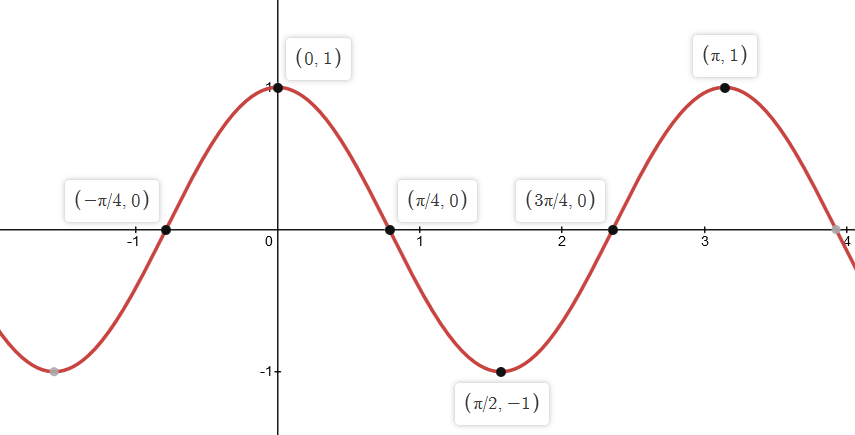
\includegraphics[scale=0.5]{Figur2.png} 
    \end{enumerate}

\end{enumerate}
\end{document}